\documentclass[a4paper,12pt, twoside]{article}
\usepackage[utf8x]{inputenc} %commentaire
\usepackage[francais]{babel} %FR
\usepackage[T1]{fontenc} 

\usepackage[pdftex]{graphicx} % img
\usepackage{wrapfig}
\usepackage{float}

\usepackage{algpseudocode}

\usepackage[top=2.5cm, bottom=2.5cm, left=2.5cm, right=2.5cm]{geometry} %Réduire les marges

% Style Page
\pagestyle{headings} % entêtes avec titres des sections en haut de pagestyle

\sloppy % ne pas faire déborder les lignes dans la marge

% Title Page
\title{
  \textbf{Mini-Rapport}
  \\[5cm]
  Exploration de la notion de méta-apprentissage
  \\[3cm]
  \textit{
  Dans quelle mesure un système apprenant peut prendre conscience de ses performances
  et altérer son comportement ?}
}


\author{
  \\[3cm]
  Yann Boniface, Alain Dutech, Nicolas Rougier \\
  Matthieu Zimmer}
  
% \date{premier semestre 2012}


\begin{document}
\maketitle


%\begin{abstract}
%\end{abstract}


%\chapter{Introduction}

%Le savoir acquis dans un réseau connexionniste reste toujours 
%de la connaissance dans le réseau plutôt que des connaissances 
%pour le réseau. 
%\newline
%Clark and Karmiloff-Smith's [Clark, A., \& Karmiloff-Smith, A. (1993)]

%Lorsqu'on est conscient de quelque chose, on est aussi conscient d'être conscient.
%\newline
%Higher-Order Thought Theory [Rosenthal, D. (1997).]

%Ces réseaux peuvent devenir extrêmement sensible à des régularités contenues dans 
%leur environnement d'entrée-sortie, mais ils n'exposent jamais la capacité à 
%accéder et manipuler cette connaissance que la connaissance. Ce savoir ne peut
%être qu'exprimé à travers l'exécution de la tâche à laquelle le réseau à était entrainé.
%\newline
%Consciousness and metarepresentation : A computational sketch
%[ Alex Cleeremans, Bert Timmermans, Antoine Pasquali . (2007)]

\newpage
\section{Introduction}

Notre intérêt s'est tourné vers l'article \cite{Cleeremans_2007} et ses 2 types de réseaux proposés.
Dans un premier temps, nous avons cherché à reproduire et expliquer les résultats
donnés, et ensuite à des solutions pour tirer profit des paris réalisés.
\newline
Nous nous sommes également penchés sur \cite{Pasquali_2010} dont nous avons reproduit
les expériences, mais leurs enjeux nous semblent encore vagues.


\section{Dupliquer le premier réseau}

\subsection{Les bases}
En premier lieu, rappelons la structure des réseaux et les résultats de l'article :
\begin{figure}[H]
\begin{center}
\begin{tabular}{cc}
 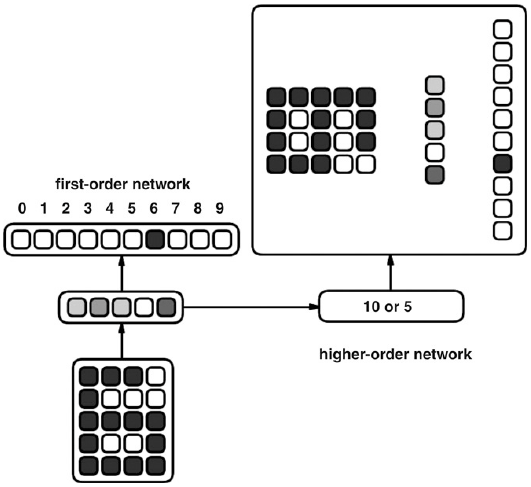
\includegraphics[width=190px]{../cleeremans_2007/digit_reco/digit_reco.png} &
 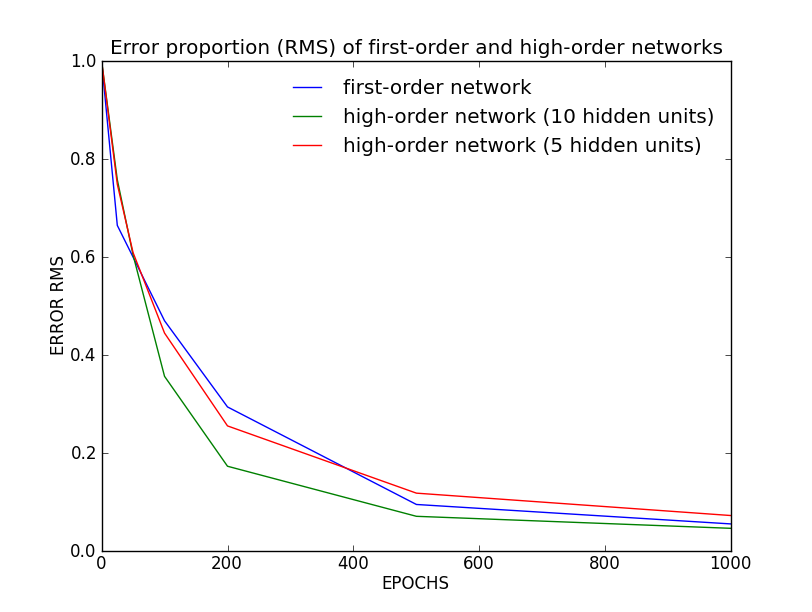
\includegraphics[width=270px]{../cleeremans_2007/digit_reco/rms.png}
\end{tabular}
\end{center}
\caption{ \cite{Cleeremans_2007} Architecture connexionniste avec méta-représentations  }
\end{figure}

La formule RMS utilisée à une époque $e$ est la suivante :
\begin{center}
\begin{large}
$ rms\ proportion_{e} = \frac{ rms_{e} = \sqrt{ \frac{1}{n} \sum \limits_{i=1}^{n} ( o_{i,e} - d_{i} )^2 }}{max(rms_{e'}),\ \forall e' \in epochs } $
\end{large}
$ with \left\lbrace \begin{array}{lll} n : number\ of\ neurons\ on\ the\ output\ layer\\o_{i,e} : value\ obtained\ for\ the\ i^{th}\ neuron\ at\ the\ e^{th}\ epoch\\d_{i} : value\ desired \ for\ the\ i^{th}\ neuron\end{array} \right.$
\end{center}

Nous avons décomposé les erreurs pour mieux comprendre le fonctionnement de l'architecture.

\begin{figure}[H]
\begin{center}
 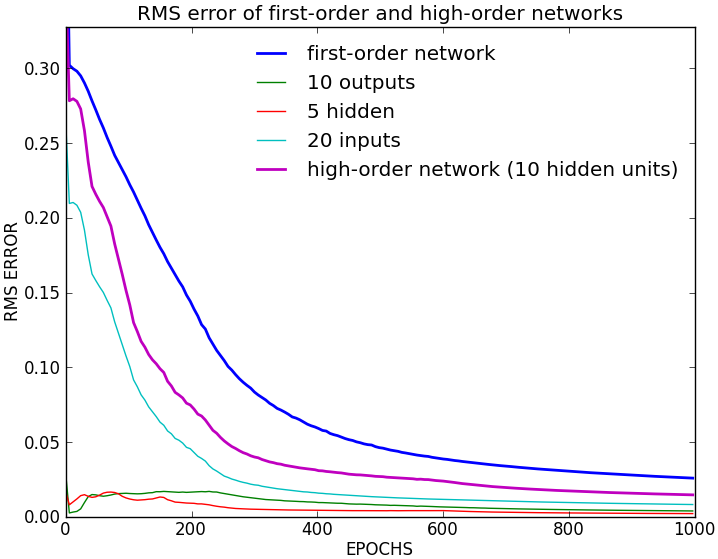
\includegraphics[width=270px]{../cleeremans_2007/digit_reco/rms_ffa.png}
\end{center}
\caption{ \textbf{Erreur RMS sans proportion}. Le réseau supérieur à 5 unités cachées n'est plus considéré, et celui à 
10 est découpé en 3 courbes pour représenter les 3 couches à reproduire. La courbe violette est donc la somme des 3 courbes des 
couches.}
\end{figure}

On peut en conclure 2 choses :
\begin{itemize}
 \item la couche caché et la couche de sortie de pose aucun problème d'apprentissage
 \item les performances du second réseau dépendent principalement de sa capacité à reproduire les entrées
\end{itemize}

Il reste une question en suspend :
\newline 
\textbf{Pourquoi le second réseau apprendrait-il plus rapidement que le premier ?}

Nous n'avons pas la réponse. Par contre, nous pouvons nous intéresser à l'erreur de classification.

\begin{figure}[H]
\begin{center}
 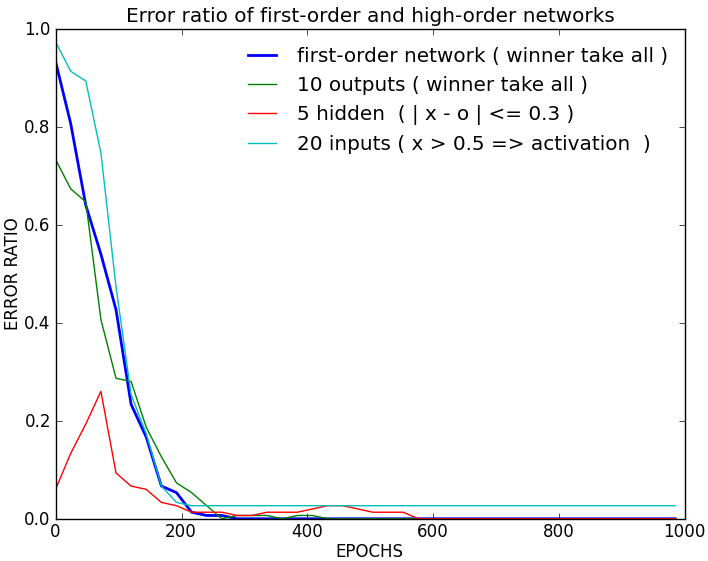
\includegraphics[width=270px]{../cleeremans_2007/digit_reco/err_ffa.png}
\end{center}
\caption{ \textbf{Erreur de classification}. Le réseau supérieur à 5 unités cachées n'est plus considéré, et celui à
10 est découpé en 3 courbes pour représenter les 3 couches à reproduire.}
\end{figure}

Il est alors beaucoup moins flagrant que le second réseau apprend mieux que le premier.
Évidemment, parler de classification de la premier couche (courbe 20 inputs) et de la couche 
caché (courbe 5 hidden) est relativement dérisoire. 
\newline La question de la rapidité d'apprentissage reste donc ouverte.

\subsection{Les rouages}

Notre attention s'est également portée sur les mécanismes qui permettaient la réalisation de cette architecture.
Nous avons alors pu remarquer que les neurones de la couche cachée du premier
réseau se stabilisaient très rapidement (autour de la 50\up{ième} époque en moyenne), le tout
permettant au second réseau d'avoir des entrées très peu variables, favorisant et permettant
donc son apprentissage.

\begin{figure}[H]
\begin{center}
 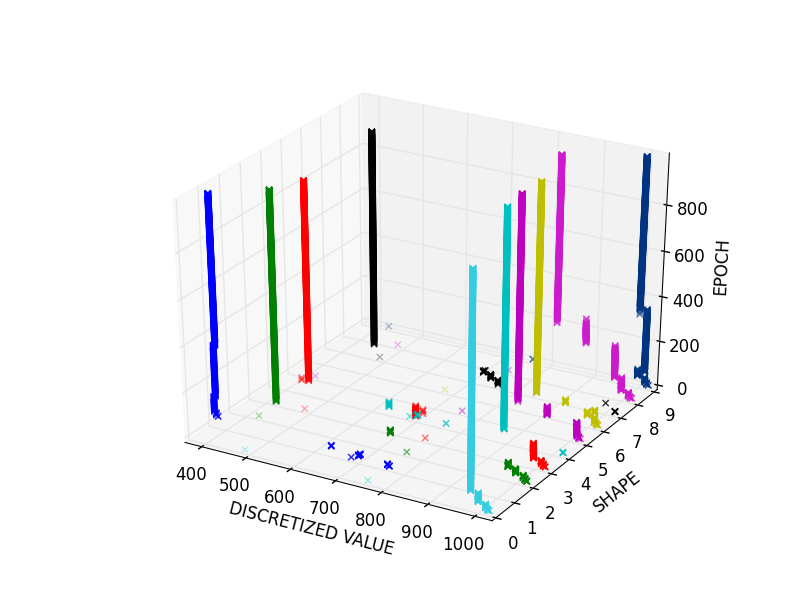
\includegraphics[height=240px]{../cleeremans_2007/digit_reco/discretize_cloud.png}
\end{center}
\caption{ Valeurs discrétisés de la couche caché du premier réseau. Chaque couleurs 
représentant un des 10 chiffres en entrée. Les courbes deviennent rapidement stables.}
\end{figure}


\subsection{Ré-haussement}

Pour revenir à l'importance des entrées, nous avons réalisé que le second réseau
n'était capable de dupliquer le premier qu'uniquement parce que ces entrées 
sont triviales.
Ainsi nous avons augmenté le nombre d'entrées en passant sur des chiffres
manuscrits \cite{Handwritten_256}, tout en augmentant proportionnellement le nombre de 
neurones des couches cachées :

\begin{figure}[H]
\begin{center}
 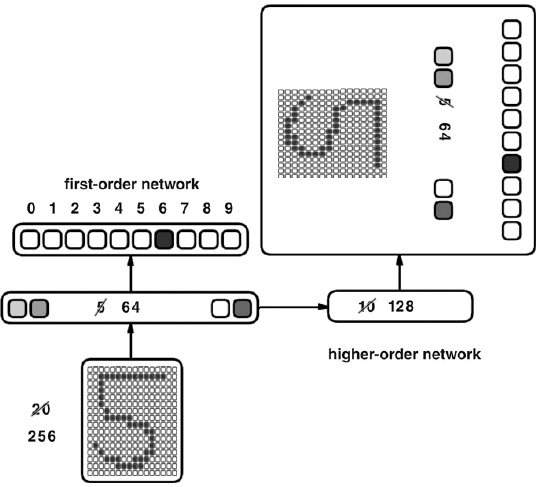
\includegraphics[height=240px]{../cleeremans_2007/digit_reco/schema_handwritten.png}
\end{center}
\caption{ Architecture avec méta-représentation pour chiffres manuscrits}
\end{figure}

Les performances du second réseau se sont alors écroulées : 
\begin{figure}[H]
\begin{center}
 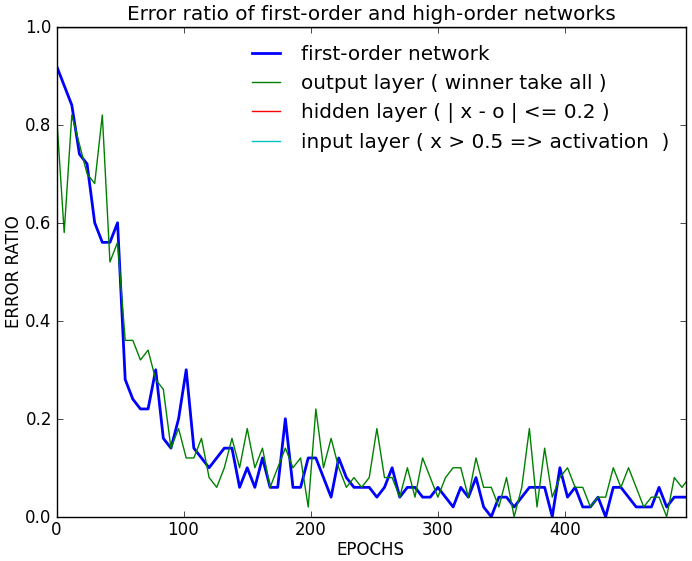
\includegraphics[height=200px]{../cleeremans_2007/digit_reco/err_handwritten.png}
\end{center}
\caption{ \textbf{Erreur de classification} de l'architecture sur des chiffres manuscrits.
L'erreur du second réseau est toujours divisé en 3.}
\end{figure}
FIXME
Il n'est alors plus capable que de reproduire la couche de sortie. Petit bémol tout de même,
le critère de classification pour la couche caché est peut-être trop rigide, il suffit qu'un
neurone diffère de 0.2 ( de la valeur voulue ) pour considérer que c'est un échec.

\newline
Tentons d'expliquer cette chute :
\newline La première chose à comprendre est que l'augmentation
du nombre de neurone n'a rien à voir avec cette perte. En effet, nous avons fait les 
simulations avec les chiffres triviales (seulement 10 formes différentes) agrandit en $16 \times 16$
et tout se passe très bien.
\newline
Cette chute provient du fait que les entrées proposées sont très nombreuses. Il s'opère ainsi
une première étape de classification dans la couche caché du premier réseau.
Donc différentes formes peuvent être représentées par la même couche cachée.
Sauf que le second réseau n'ayant en entrée que la version factorisé (la couche caché), il lui 
est impossible de retrouver les formes initiales.


\subsection{Représentations}

Enfin, nous avons remarqué qu'en bloquant l'apprentissage entre la couche cachée et les 
entrées du premier réseau, puis en changeant de tâche, le réseau était capable de réapprendre
la nouvelle tâche, ce qui prouve bien la présence d'une représentation des entrées dans la couche 
cachée.

\begin{figure}[H]
\begin{center}
 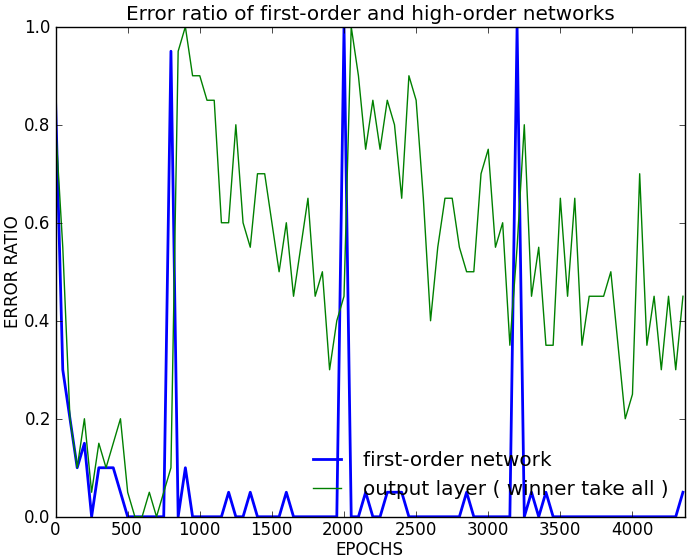
\includegraphics[height=200px]{../cleeremans_2007/digit_reco/err_handwritten_relearn_2.png}
\end{center}
\caption{ \textbf{Erreur de classification} de l'architecture sur des chiffres manuscrits.
Apprentissage bloqué à l'époque 800. Changement de tâche aux époques : 800, 2000, 3200}
\end{figure}

\subsection{Remarque}

Il faut cependant remarquer qu'un simple perceptron est suffisant pour réaliser la tâche
du premier réseau (même sur les chiffres manuscrits), et donc, qu'il est possible que 
dans le cas d'un problème non linéairement séparable cette architecture soit invalidée.
 
\begin{figure}[H]
\begin{center}
 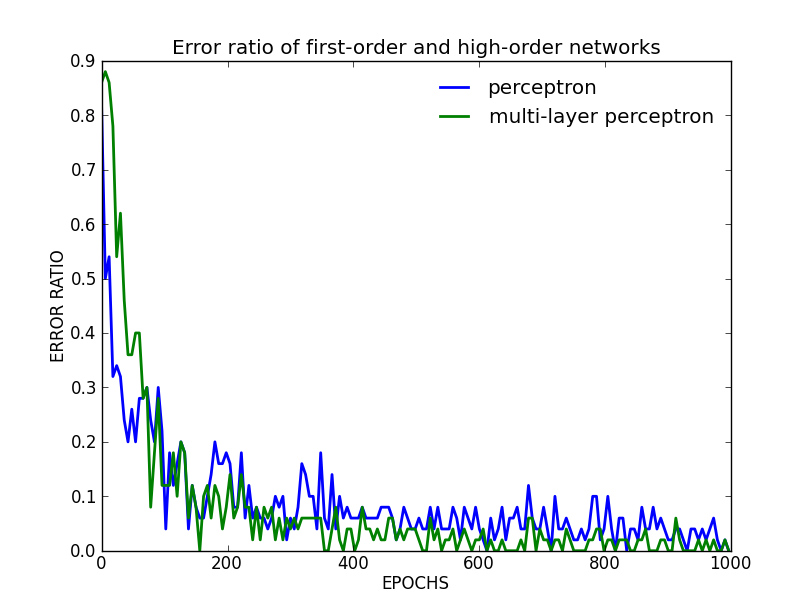
\includegraphics[height=230px]{../cleeremans_2007/digit_reco/p_vs_mlp.png}
\end{center}
\caption{ \textbf{Erreur de classification} d'un perceptron et d'un perceptron multi-couches
sur la base de chiffres manuscrits.}
\end{figure}

\section{Parier sur le premier réseau}

\subsection{Les bases}

Rappelons également la structure des réseaux et les résultats :
\begin{figure}[H]
\begin{center}
\begin{tabular}{cc}
 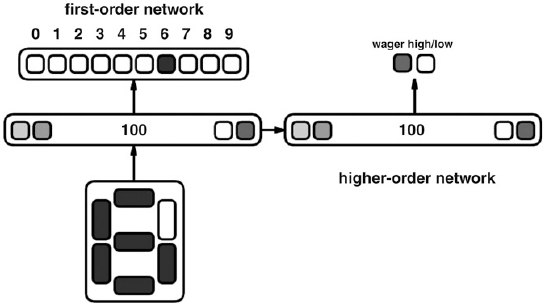
\includegraphics[width=220px]{../cleeremans_2007/digital_reco/schema.png} &
 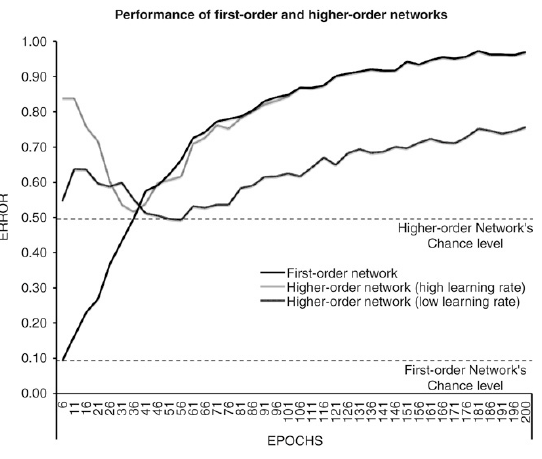
\includegraphics[width=220px]{../cleeremans_2007/digital_reco/perf_article.png}
\end{tabular}
\end{center}
 \caption{ \cite{Cleeremans_2007}  Architecture connexionniste avec paris  }
\end{figure}


La première chose que nous avons faites à été d'améliorer les performances du second réseau
en modifiant quelques paramètres (initialisation des poids sur [-1 ; -1], momentum à 0.5). 

\begin{figure}[H]
\begin{center}
\begin{tabular}{cc}
 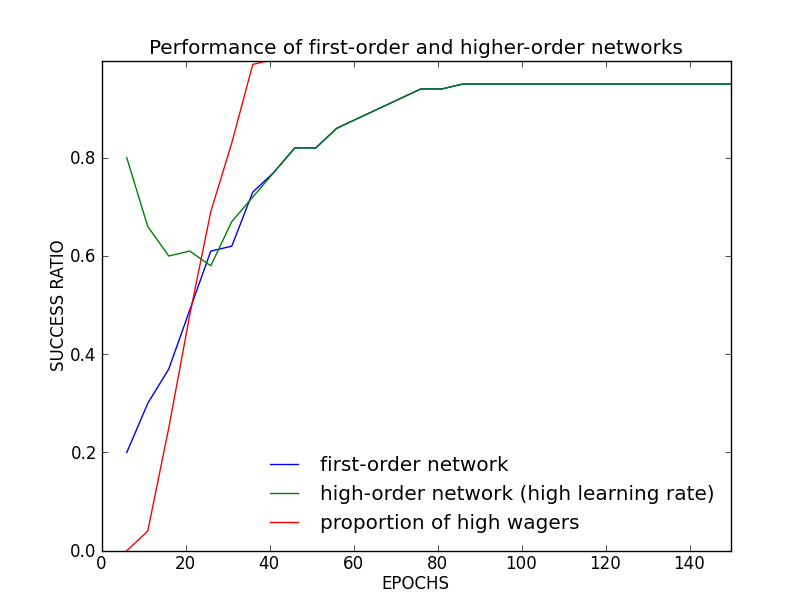
\includegraphics[width=230px]{../cleeremans_2007/digital_reco/perf_wag.png} &
 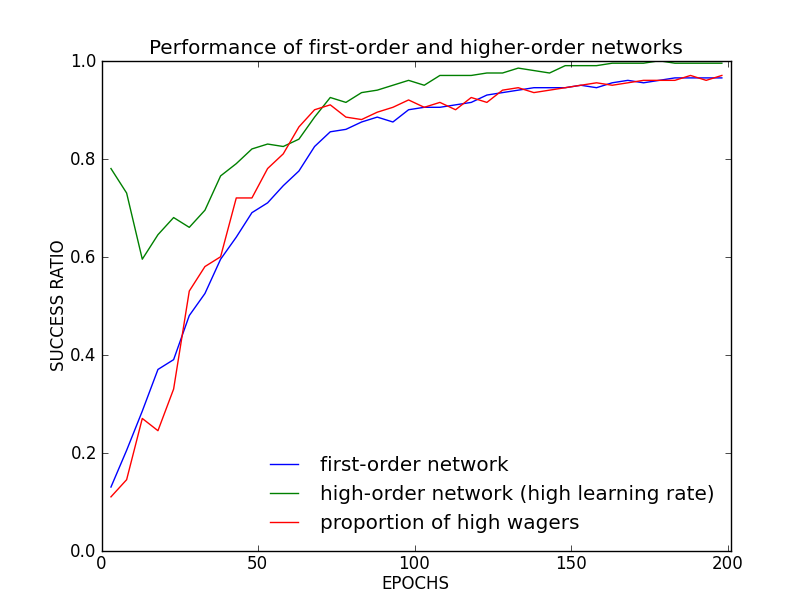
\includegraphics[width=230px]{../cleeremans_2007/digital_reco/perf_boost.png}
\end{tabular}
\end{center}
 \caption{ Performance de l'architecture. À gauche la base, à droite la version améliorée.
 On ne considère plus le réseau avec apprentissage faible, mais on a ajouté le taux de paris hauts.}
\end{figure}

Contrairement à celui de l'article, il ne se contentera 
plus simplement de parier haut à chaque coups (après 40 époques). Il aura une longueur d'avance
sur le premier réseau sur toute la durée de l'apprentissage. On pourra donc tirer profit de
cette avance.

\subsection{Feedbacks}

À partir de cette différence de performances, nous avons imaginé plusieurs architectures, qui
améliorent plus ou moins les performances de reconnaissance du réseau sur des chiffres manuscrits:

\begin{figure}[H]
 \begin{center}
\begin{tabular}{c|c}
 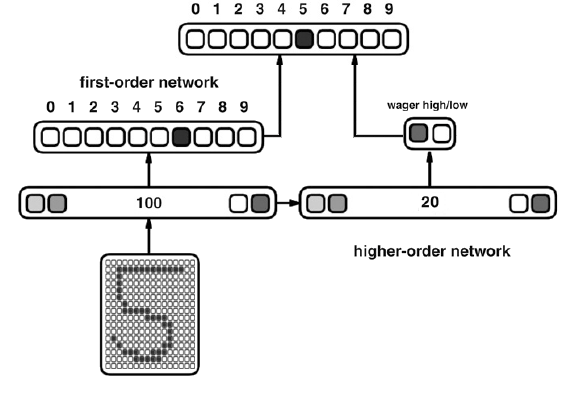
\includegraphics[width=210px]{../pre-presentation/thrid.png} & 
 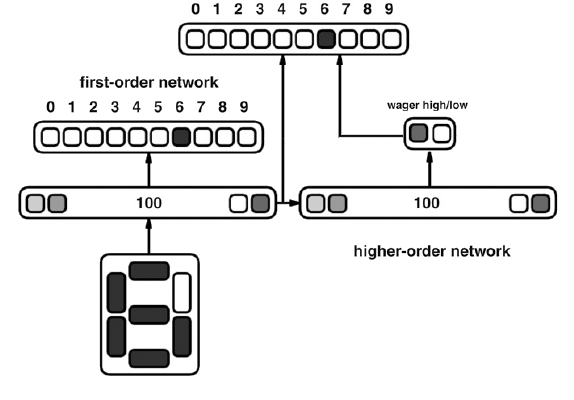
\includegraphics[width=210px]{../pre-presentation/thrid_hidden.png}
\end{tabular}
\end{center}
\caption{Architecture avec 3\up{ième} réseau}
\end{figure}

Dans ces 2 architectures, nous nous contentons de connecter un 3\up{ième} réseau qui doit 
tirer des conclusions à partir d'informations sur les 2 premiers.

\begin{figure}[H]
 \begin{center}
 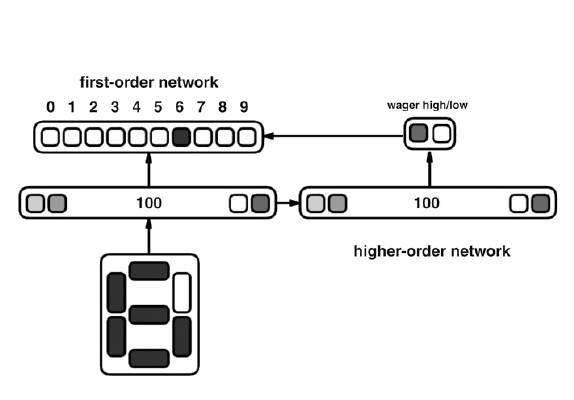
\includegraphics[width=250px]{../pre-presentation/merging.png}
\end{center}
\caption{Architecture par fusion}
\end{figure}

Ici, nous mélangeons un apprentissage par descente de gradient (sur le premier et second réseau)
et un apprentissage perceptron (entre les 2 couches de sorties).

\begin{figure}[H]
 \begin{center}
 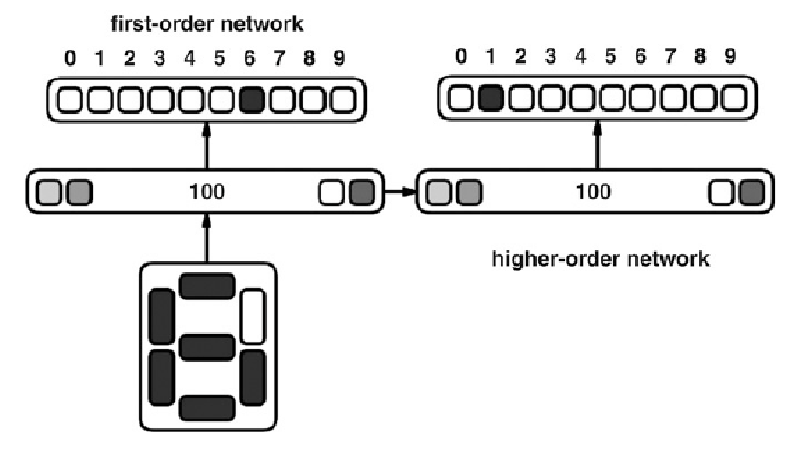
\includegraphics[width=300px]{../pre-presentation/nth_wta.png}
\end{center}
\caption{Architecture par intuitions}
\end{figure}

Cette architecture est légèrement différente dans le sens où elle n'enregistre
plus de pari mais l'indice du n\up{ième} neurone le plus actif contenant la bonne réponse.
Exemple : le réseau supérieur sort 2 -> la réponse est le 3\up{ième} neurone le plus actif 
de la couche de sortie du premier réseau.
\newline

Nous avons aussi essayé quelques modèles où le réseau supérieur servait de superviseur
à l'apprentissage du premier réseau. Par exemple, s'il parie haut, l'apprentissage du premier réseau
sera faible, sinon il sera accentué.

\section{La suite}

Ce que nous continuons d'étudier : 
\begin{itemize}
 \item validation sur des expériences plus complexes (qui ne peuvent être résolue directement par un perceptron)
 \item relation entre la taille de la couche cachée du premier réseau et le taux de paris avantageux
 \item nouveau critère de classification pour la couche caché dans la première architecture sur les chiffres manuscrits
 \item approfondir les intérêts du second article \cite{Pasquali_2010}
 \item de nouvelles architectures axées méta-apprentissage où le réseau d'ordre supérieur contrôle le premier
 (taux d'apprentissage, momentum, entrées à approfondir, ...) telle une conscience
\end{itemize}


\bibliographystyle{apalike}
\bibliography{biblio}

\newpage
\appendix
\section{Algorithme}

Ensemble d'inscrutions executé pour une époque et un tirage d'entrées/sorties.
\newline
Cet algorithme se déroule en plusieurs temps :
\begin{itemize}
 \item[a] On calcule la sortie du premier réseau en ignorant le second ( valeur à 0 )
 \item[b] On calcule la sortie du second réseau
 \item On calcule la sortie du premier réseau avec les sorties de b)
\end{itemize}


\begin{algorithmic}

\State $first\_order.calc\_hidden\_layer(samples.inputs)$
\State $high\_order.calc\_output\_layer(first\_order.hidden\_layer)$
\State $first\_order.calc\_output\_layer(first\_order.hidden\_layer,\ [0, ..., 0])$
\State 
\State $h\_output \gets ampli(high\_order.output\_layer)$
\State $right\_houtput \gets [0,\ 0]$
\If{$good\_answer(first\_order)$}
  \State $right\_houtput[1] \gets 1$
\Else
  \State $right\_houtput[0] \gets 1$
\EndIf
\State $first\_order.calc\_output\_layer(first\_order.hidden\_layer,\ h\_output)$
\State
\State $calc\_stats()$
\State
\State $high\_order.train(first\_order.hidden\_layer,\ right\_houtput)$
\State $first\_order.train(samples.inputs,\ samples.outputs,\ h\_output)$


\end{algorithmic}

L'interêt se porte sur

\begin{algorithmic}

\Function{$train$}{$inputs,\ outputs,\ add$}
\For {$i = 0 \to output\_neurons.length$}
\State $y_{output}[i] \gets g'(output\_neurons[i].a) \times ( outputs[i] - output\_neurons.state )$
\EndFor
\\
\For {$i = 0 \to hidden\_neurons.length$}
\State $w\_sum \gets \sum \limits_{j=0}^{output\_neurons.length} output\_neurons[j].weights[i] \times y_{output[j]}$
\State $y_{hidden}[i] \gets g'(hidden\_neurons[i].a) \times w\_sum$
\EndFor
\State $update\_weights\_hidden\_layer(y_{hidden})$
\\
\For {$i = 0 \to output\_neurons.length$ } 
\State $output\_neurons[i].update\_weights\_gradient(y_{output}[i],\ hidden\_neurons,\ add)$
\State $output\_neurons[i].update\_weights\_perceptron(outputs[i],\ hidden\_neurons,\ add)$
\EndFor
\EndFunction

\end{algorithmic}


\begin{algorithmic}

\Function{$update\_weights\_gradient$}{$error,\ intputs,\ add$}
\State $calc\_output(inputs + add)$
\\
\For {$j = 0 \to inputs.length$ } 
\State $dw \gets weights[j] - last\_weights[j]$
\State $p \gets error \times inputs[j]$
\State $weights[j] \gets weights[j] + learning\_rate \times p + momentum \times dw$
\EndFor
\EndFunction

\end{algorithmic}


\begin{algorithmic}

\Function{$update\_weights\_perceptron$}{$goal,\ intputs,\ add$}
\State $calc\_output(inputs + add)$
\\
\For {$j = inputs.length \to inputs.length + add.length$ } 
\State $dw \gets weights[j] - last\_weights[j]$
\State $p \gets (goal - state ) \times add[inputs.length - j]$
\State $weights[j] \gets weights[j] + \frac{learning\_rate \times p + momentum \times dw}{add.length} $
\EndFor
\EndFunction

\end{algorithmic}

\end{document}



